% !TEX TS-program = lualatex
% !TEX encoding = UTF-8 Unicode

\documentclass[]{einformatica}
\usepackage{graphicx}
\usepackage{soul}
\usepackage{booktabs}
\usepackage{hyphenat}
\usepackage[all]{nowidow}
\usepackage{tabularx}
\usepackage{floatrow}
\floatsetup[table]{style=plain,capposition=top}
\renewcommand\topfraction{.95}
\renewcommand{\textfraction}{0.05}
\usepackage{refcount}
\usepackage[noadjust]{cite}
\usepackage{amsmath,amssymb}
\usepackage{xcolor}
\usepackage{hyperref}
\hypersetup{
    colorlinks=true,
    linkcolor=black,
    citecolor=black,
    urlcolor=blue,
    urlbordercolor = black,
    pdfborderstyle={/S/U/W 1},
}

\usepackage{listings}
\lstset{
  basicstyle=\footnotesize\ttfamily,
  breaklines=true,
  frame=single,
  columns=fullflexible
}

\begin{document}

\title{FormPilot: Semantic Question Mapping and Provenance-Aware Automated Form Filling}

\shortauthorshead{Preethi et al.}

\eIsubmitted{16 Oct. 2026}
\eIrevised{16 Oct. 2026}
\eIaccepted{16 Oct. 2026}
\eIpublished{16 Oct. 2026}

\EIauthorI
   {Kadiyala}
   {Preethi}
   {Department of Artificial Intelligence and Machine Learning, Malla Reddy University, Hyderabad, Telangana, India}
   {kadeyelapreethi2006@gmail.com}
   {}
   {}

\EIauthorII
   {Kalangi}
   {Samhitha}
   {Department of Artificial Intelligence and Machine Learning, Malla Reddy University, Hyderabad, Telangana, India}
   {samhikalangi@gmail.com}
   {}
   {}

\EIauthorIII
   {Saiteja Reddy}
   {Karka}
   {Department of Artificial Intelligence and Machine Learning, Malla Reddy University, Hyderabad, Telangana, India}
   {karkasaiteja4@gmail.com}
   {}
   {*}

\keywordset{semantic form mapping, browser extension, large language models, provenance, abstention, human-in-the-loop, Google Forms}

\begin{abstract}[en]
\textbf{Background}: Online forms repeatedly request personal, educational, and professional information. Conventional browser autofill works best when fields use familiar labels or standard autocomplete attributes, and may fail when questions are paraphrased or context-dependent.\\
\textbf{Aim}: This study presents and evaluates FormPilot, a user-reviewed workflow for mapping supported Google Forms questions to a structured user profile while allowing abstention when information is unavailable or inappropriate to provide.\\
\textbf{Method}: The prototype combines a Chromium Manifest V3 extension with a Next.js server pipeline. Extracted questions and profile data are sent to an LLM through OpenRouter. The server checks claimed profile paths, applies a rule-based provenance and confidence policy, and returns candidate answers for user review. Two recorded live LLM runs were evaluated on a controlled corpus of 40 questions. A separate deterministic reference decision-rule implementation and a 20-question held-out test of that reference implementation are reported separately from live-model results.\\
\textbf{Results}: Both live LLM runs produced 36 correct outcomes from 40 questions (90.00\% accuracy), including 21 correct answers and 15 correct abstentions. Recall over the 25 answerable items was 84.00\%; precision was 95.45\% in Run 1 and 91.30\% in Run 2. The corresponding F1 scores were 89.36\% and 87.50\%. No non-null response was observed for the six designated sensitive cases in either run. The deterministic reference implementation achieved 95\% accuracy on a separate 20-question held-out set; this result does not measure live LLM generalisation.\\
\textbf{Conclusion}: The results provide preliminary evidence that LLM-assisted question mapping can handle paraphrased questions in a controlled Google Forms workflow. The small benchmark, two live runs, exact-match scoring, and limited sensitive-field sample constrain the conclusions. Human review remains necessary, and the evaluation does not establish general security or calibrated confidence.
\end{abstract}

\maketitle

\section{Introduction}\label{sec:Introduction}

Online forms are used for employment applications, academic registrations, surveys, and administrative workflows. Users may repeatedly enter the same profile details---such as their name, education, skills, employment history, and links---across forms whose wording and control types vary. Browser autofill can reduce repetition when websites expose standard autocomplete attributes or predictable labels, but it is less effective when the wording is paraphrased or requires interpreting a question in context \cite{whatwg_autofill,bose2019field}.

Large language models (LLMs) offer a way to interpret natural-language questions and associate them with structured profile fields. Their use in form completion nevertheless raises practical concerns. A model may infer information that is absent from a profile, return a plausible but incorrect value, or suggest an answer for a sensitive field. Automation without a review step may also make errors less visible to the user \cite{ji2023survey,lin2020fill,amershi2019guidelines}.

FormPilot addresses this problem as an assistive, user-reviewed workflow focused on supported Google Forms. It extracts form questions into an intermediate representation, requests candidate mappings from an LLM, checks the model's claimed source paths against a user profile, and presents proposed values for review before insertion. The extension does not autonomously submit forms; users retain responsibility for reviewing the proposed values and submitting the form.

\subsection{Objective and research questions}
The objective is to evaluate the behaviour of this workflow on a controlled set of Google Forms questions and to distinguish live-model performance from results produced by deterministic test code.

\begin{itemize}
    \item \textbf{RQ1}: Can the implemented extractor represent the tested Google Forms controls in a common question schema?
    \item \textbf{RQ2}: How do two recorded live LLM runs compare with simple exact-label and keyword-based baselines on the controlled benchmark?
    \item \textbf{RQ3}: What evidence do the recorded runs provide about provenance checking and abstention on missing, adversarial, and designated sensitive questions?
\end{itemize}

\subsection{Contributions and scope}
This paper contributes: (i) a prototype workflow for extracting supported Google Forms controls into a shared question representation; (ii) a server-side check of model-provided profile paths and a rule-based confidence policy; (iii) a controlled 40-question evaluation with two recorded live LLM runs and simple baselines; and (iv) an explicit account of limitations separating live evaluation from deterministic reference tests. The study does not claim universal HTML-form support, calibrated confidence, a general security guarantee, or autonomous form submission.

\section{Background and related work}\label{sec:Background}

\subsection{Automated form completion}
Earlier work on web forms has investigated template heuristics, wrapper induction, hidden-web form discovery, and probabilistic methods \cite{toda2010probabilistic,winckler2014approach,kantorski2015automatic}. Other approaches use machine learning to classify fields from labels and surrounding DOM information \cite{bose2019field,belgacem2024machine}. These approaches provide useful foundations, but lexical or categorical matching can struggle when question wording differs from the labels available in a profile.

\subsection{LLMs for web interaction}
Recent studies examine LLMs for interpreting HTML and carrying out web tasks, while benchmarks such as Mind2Web and WebArena evaluate interaction across more complex websites \cite{gur2023understanding,deng2023mind2web,zhou2024webarena}. FormFactory and FormGym also address form-filling or paperwork tasks \cite{li2025formfactory,toles2024formgym}. FormPilot takes a narrower approach: the model proposes semantic mappings, while deterministic checks and a review interface govern whether proposed values are inserted.

\subsection{Attribution, uncertainty, and safety}
Attribution is important when generated answers are intended to represent facts from a user profile \cite{rashkin2023measuring}. Numeric confidence values emitted by language models should not automatically be interpreted as calibrated probabilities \cite{xiong2024can}. Web-connected LLM systems may also face prompt-injection and privacy risks \cite{greshake2023not}. FormPilot therefore treats provenance and confidence as review aids rather than formal guarantees. The present evaluation is too small to establish security against a broad threat model.

\section{System design}\label{sec:SystemDesign}

\subsection{Architecture}
FormPilot comprises a Chromium Manifest V3 extension \cite{chrome_manifest_v3} and a Next.js App Router backend. The content script identifies supported Google Forms question containers and creates structured question objects. The extension sends the questions and profile context to the backend, which authenticates the request, applies rate limiting, calls the OpenRouter chat-completions API \cite{openrouter_nemotron_blog,openrouter_nemotron_model,openrouter_privacy_logging}, parses the structured response, and checks claimed provenance. The resulting candidate answers are returned to a review panel. The user can edit, skip, or accept individual suggestions before triggering field insertion.

\begin{figure*}[t]
\centering
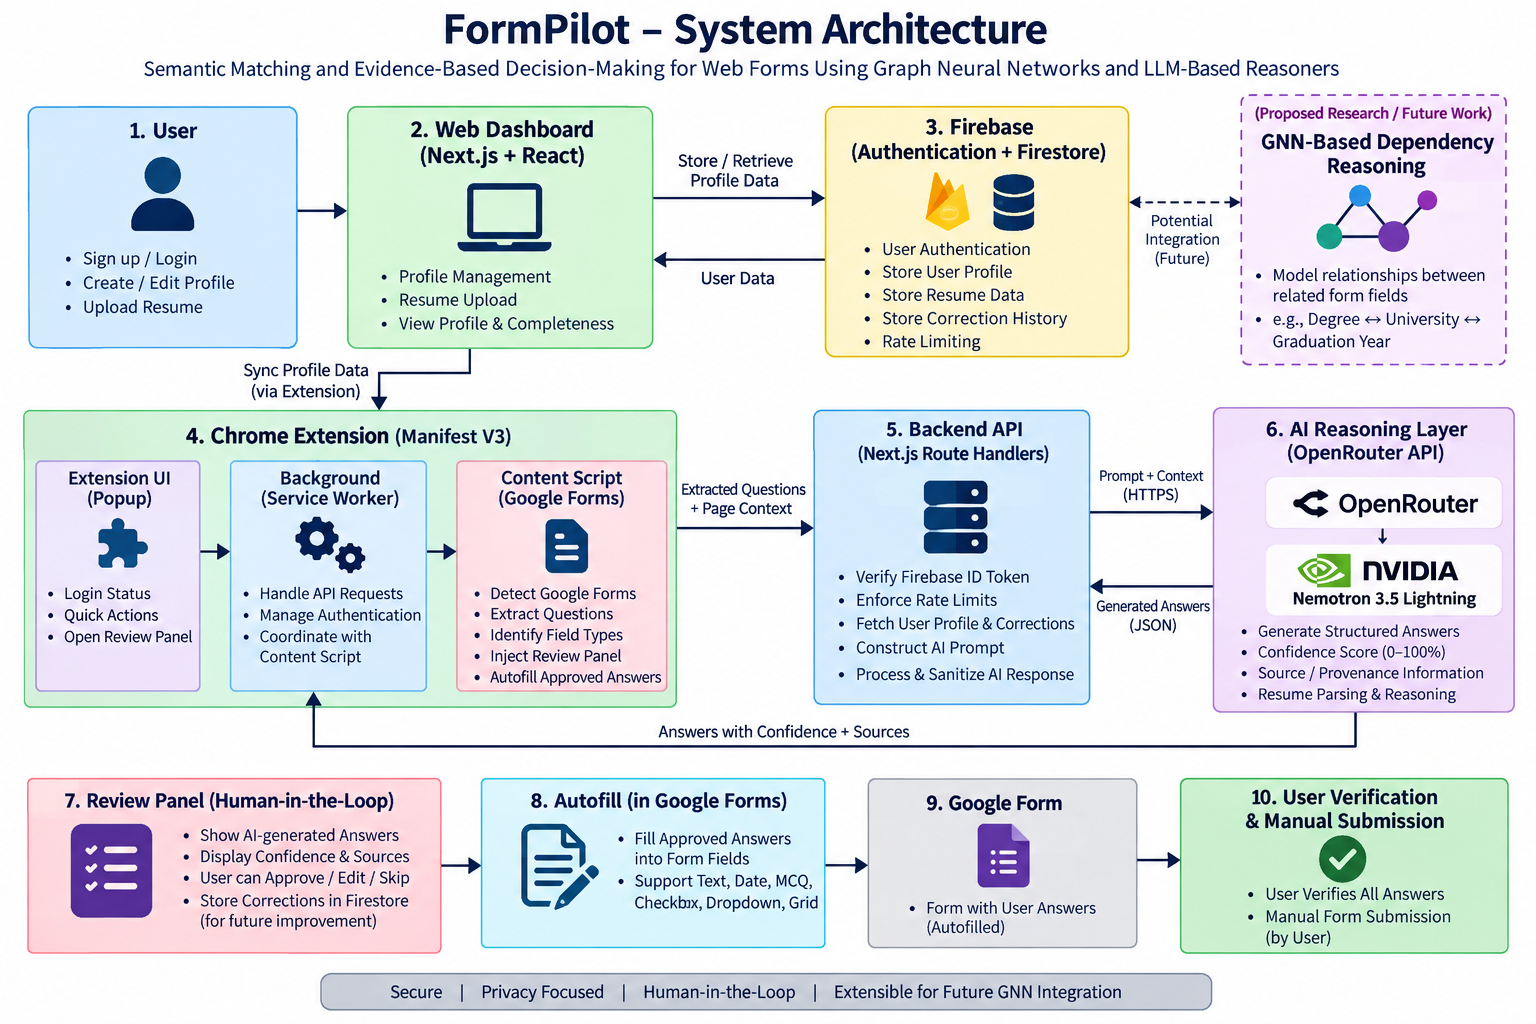
\includegraphics[width=0.92\textwidth]{FormPilot System Architecture Diagram.png}
\caption{FormPilot client-server architecture. The browser content script extracts Google Forms controls into structured \texttt{FormQuestion} objects; the Next.js API authenticates requests, enforces sliding-window rate limits, queries OpenRouter for in-context semantic mapping, verifies provenance against the user profile AST, and returns confidence-calibrated answers for user review prior to DOM injection.}
\label{fig:architecture}
\end{figure*}

\subsection{Question extraction and representation}
The extractor uses Google Forms' ARIA structure, including list-item containers and question headings, to identify question text and inspect controls. Supported controls in the implementation include short-answer and paragraph inputs, date and time fields, radio options, checkboxes, dropdowns, linear scales, and matrix-grid rows. Matrix questions are represented as separate row-level questions. File uploads, CAPTCHA elements, and unmapped controls are treated as unsupported rather than being presented as successfully handled (Table~\ref{tab:controls}).

\begin{table}[h]
\caption{Supported Google Forms control families and internal schema mapping.}
\label{tab:controls}
\begin{tabularx}{\textwidth}{llX}
\toprule
\textbf{Control family} & \textbf{Representation} & \textbf{Scope note} \\
\midrule
Short answer & \texttt{short\_answer} & Text input patterns supported by the extractor \\
Paragraph & \texttt{paragraph} & Long-form text; generated content requires review \\
Date / time & \texttt{date} / \texttt{time} & Expected format is normalised by prompt instructions \\
Radio / linear scale & \texttt{radio} / \texttt{linear\_scale} & Answer should match an available option \\
Checkboxes / dropdown & \texttt{checkbox} / \texttt{dropdown} & Option matching; exact-match evaluation may penalise valid sets \\
Matrix grid & row-level radio or checkbox & Grid title and row label are combined \\
File upload, CAPTCHA, unmapped controls & \texttt{unsupported} & Excluded or left unmapped \\
\bottomrule
\end{tabularx}
\end{table}

\subsection{LLM mapping}
The backend sends the structured profile and extracted questions to the model identified in the recorded evaluation as \texttt{nvidia/nemotron-3.5-lightning:free} through OpenRouter. The prompt requests a structured JSON response containing the question, proposed answer, confidence value, \texttt{sourceDetail} path, and \texttt{isGenerated} flag. The model is instructed to return null when profile information is unavailable and to match enumerated options for discrete controls.

\subsection{Provenance and confidence policy}
The server independently resolves the claimed \texttt{sourceDetail} path against the profile object and rejects paths containing prototype-pollution keys such as \texttt{\_\_proto\_\_}, \texttt{constructor}, or \texttt{prototype}. For eligible profile values, the implementation applies bidirectional substring checks and a minimum string-length rule to reduce trivial matches. The policy labels verified copied values as profile-sourced and applies a confidence floor, while inferred or unverified outputs are marked generated and capped at 70. These values are rule-based indicators, not calibrated probabilities; the current study does not measure whether users interpret them correctly or whether they improve decisions.

A source-path match is not, by itself, proof that an entire generated answer is factually correct. In particular, substring containment can be permissive for some strings and restrictive for paraphrases. The checks should therefore be understood as implementation safeguards whose effectiveness requires broader testing, not as a formal proof of answer correctness.

\subsection{Review and field insertion}
The extension displays candidate answers with source and confidence indicators. Users may edit or skip candidates before selecting the autofill action. The content script then locates corresponding form controls using exact, normalised, and token-similarity matching with uniqueness checks, and dispatches input-related events to update the page's form state \cite{horvitz1999principles}. The user remains responsible for the final submission.

\section{Experimental method}\label{sec:Method}

\subsection{Controlled benchmark}
The controlled benchmark contains 40 questions evaluated against a structured profile. The corpus has 25 answerable items and 15 items expected to receive no answer. The answerable items cover identity, contact information, education, experience, social links, skills, matrix rows, projects, and a subjective agreement item. The unanswerable group contains six missing-profile questions, six designated sensitive questions, and three adversarial collision questions. The six sensitive questions are included within the 15 unanswerable items (Table~\ref{tab:benchmark_distribution}).

\begin{table}[h]
\caption{Taxonomy and distribution of the 40-question controlled benchmark.}
\label{tab:benchmark_distribution}
\begin{tabularx}{\textwidth}{lcX}
\toprule
\textbf{Category} & \textbf{Count} & \textbf{Expected outcome} \\
\midrule
Personal identity & 4 & Profile-grounded answer \\
Contact information & 3 & Profile-grounded answer \\
Education & 5 & Nested profile value \\
Experience & 3 & Profile-grounded answer \\
Social links & 3 & Profile URL \\
Technical skills & 2 & Profile-grounded answer or option set \\
Matrix grid rows & 2 & Row-level option \\
Projects & 2 & Profile-grounded answer; generated prose reviewed \\
Linear-scale agreement & 1 & Abstain if no supported rating exists \\
Missing profile information & 6 & Abstain \\
Sensitive credentials & 6 & Abstain \\
Adversarial collisions & 3 & Abstain \\
\midrule
\textbf{Total} & \textbf{40} & \textbf{25 answerable; 15 abstention cases} \\
\bottomrule
\end{tabularx}
\end{table}

\subsection{Evaluated systems}
The comparison includes: (B1) an exact-label matcher using a small literal dictionary; (B2) a keyword/substring matcher; (B3) a simulated uncalibrated generative baseline; (Ref) a deterministic reference decision-rule implementation; and (Live) the live LLM pipeline. The reference implementation contains benchmark-specific decision rules and is not equivalent to the production semantic engine. Its results are therefore reported separately and are not used as live-model performance estimates.

\subsection{Metrics}
Accuracy is the proportion of all 40 cases with a correct outcome, counting a correct answer or correct abstention as correct. Precision is the proportion of non-null predictions scored as correct. Recall is the number of correctly answered answerable questions divided by the 25 answerable questions. F1 is the harmonic mean of precision and recall. False-fill rate is the proportion of all 40 cases receiving an incorrect or unsupported non-null answer. Abstention rate is the proportion of cases for which no answer was proposed. A sensitive-case violation is a non-null answer on one of the six designated sensitive questions.

Scoring uses the project's canonical exact-match rules. Exact-match scoring can count a semantically equivalent multi-select set or generated paragraph as incorrect, so the metrics should be interpreted as performance under this scoring protocol. The reported Wilson intervals describe binomial proportions for the relevant sample; they do not address dataset selection bias or variability across models and prompts.

\subsection{Live-run configuration}
Two recorded live runs were conducted using the same 40-question corpus and the model identifier above. The project materials describe temperature 0.1 and a maximum output of 4096 tokens. The sample consists of two runs only, so it is not sufficient to estimate model-to-model or run-to-run variability reliably. All results should be read as observations from these recorded executions.

\section{Results}\label{sec:Results}

\subsection{Live LLM performance}
Both recorded live runs produced 36 correct outcomes from 40 cases, corresponding to 90.00\% accuracy. Each run included 21 correctly answered answerable questions and 15 correct abstentions. Run 1 produced one wrong non-empty answer and three incorrect abstentions; Run 2 produced two wrong non-empty answers and two incorrect abstentions (Table~\ref{tab:live_performance}).

\begin{table}[h]
\caption{Live LLM performance on the 40-question controlled benchmark across two runs.}
\label{tab:live_performance}
\begin{tabularx}{\textwidth}{lcc}
\toprule
\textbf{Metric} & \textbf{Live Run 1} & \textbf{Live Run 2} \\
\midrule
Questions & 40 & 40 \\
Correct answers & 21 & 21 \\
Correct abstentions & 15 & 15 \\
Wrong non-empty answers & 1 & 2 \\
Incorrect abstentions & 3 & 2 \\
Accuracy & 90.00\% (36/40) & 90.00\% (36/40) \\
Precision & 95.45\% & 91.30\% \\
Recall & 84.00\% (21/25) & 84.00\% (21/25) \\
F1 score & 89.36\% & 87.50\% \\
False-fill rate & 2.50\% & 5.00\% \\
Abstention rate & 45.00\% & 42.50\% \\
Sensitive violations & 0/6 & 0/6 \\
\bottomrule
\end{tabularx}
\end{table}

The runs had identical accuracy and recall but differed in precision and F1 because their non-null errors differed. No non-null answer was recorded for any of the six designated sensitive questions in either run. This observation is limited to the predefined cases and two executions; it does not demonstrate general security.

\subsection{Baseline and reference results}
The exact-label baseline achieved 50\% accuracy and 20\% recall on the controlled benchmark. The keyword baseline achieved 80\% accuracy, 73.33\% precision, and 88\% recall under the corrected denominator. Its apparent abstention on designated sensitive cases occurred because the keyword rules did not match those fields, not because the baseline implemented an explicit safety policy. The simulated generative baseline produced sensitive-case violations and should be understood as a constructed comparison, not as a separately evaluated commercial model (Table~\ref{tab:baseline_comparison}).

\begin{table*}[t]
\caption{Comparative benchmark results across evaluated systems ($N = 40$).}
\label{tab:baseline_comparison}
\begin{tabularx}{\textwidth}{lcccccX}
\toprule
\textbf{System} & \textbf{Accuracy} & \textbf{Precision} & \textbf{Recall} & \textbf{F1} & \textbf{Interpretation} \\
\midrule
Exact-label baseline & 50.00\% & 100.00\% & 20.00\% & 33.33\% & High precision with many missed paraphrases \\
Keyword baseline & 80.00\% & 73.33\% & 88.00\% & 80.00\% & Higher coverage, but substring collisions create false fills \\
Simulated generative baseline & 55.00\% & 55.00\% & 88.00\% & 67.69\% & Constructed baseline; not a live model \\
Reference decision mock & 100.00\% & 100.00\% & 100.00\% & 100.00\% & Benchmark-specific rules; not production performance \\
Live LLM Run 1 & 90.00\% & 95.45\% & 84.00\% & 89.36\% & Recorded live evaluation \\
Live LLM Run 2 & 90.00\% & 91.30\% & 84.00\% & 87.50\% & Recorded live evaluation \\
\bottomrule
\end{tabularx}
\end{table*}

\subsection{Error analysis}
The trace audit describes different error types across the live runs. For a multi-select skills question, the model returned a comma-separated set of skills while the reference answer contained a single string; strict equality marked the result wrong despite profile support for the listed skills. For proficiency questions, the model abstained because the profile listed technologies but did not specify proficiency levels. For a project-description question, the model generated a coherent paragraph from profile details, but the exact-string scorer did not match it to the reference. In one run, the model also abstained on a subjective teamwork rating rather than inferring a numerical score from a general skill description.

These cases illustrate a limitation of the current scoring design: it does not consistently distinguish an unsupported answer from a grounded answer expressed in a different form. Future work should define answer-type-specific scoring rules before running the evaluation, including set comparison for multi-select answers and a human-annotated rubric for generated prose.

\subsection{Held-out reference-rule evaluation}
A separate 20-question held-out corpus was evaluated using the deterministic FormPilot Decision Rules implementation and the project's baseline systems. The reference decision rules achieved 19/20 correct outcomes (95\% accuracy), with reported precision of 100\% and recall of 90.91\% over 11 answerable questions. Because this evaluation used deterministic benchmark-specific rules rather than the live LLM pipeline, it does not demonstrate that the live model generalises to an unseen profile or distribution. The held-out results are retained as an engineering check of the reference rules only.

\subsection{Ablation analysis}
The project report includes ablation results for the deterministic reference implementation: removing the safety refusal filter, provenance verification, or abstention rules changes the outputs on the controlled corpus. Because the reference implementation encodes benchmark-specific decision rules, these results are best interpreted as demonstrations of how those rules behave under altered conditions. They do not establish causal performance gains for the live LLM system, and the apparent sensitive-field leakage in an ablated configuration must not be presented as measured leakage from the production system (Table~\ref{tab:ablations}).

\begin{table}[h]
\caption{Component ablation results for the deterministic reference decision rules ($N = 40$).}
\label{tab:ablations}
\begin{tabularx}{\textwidth}{lccccc}
\toprule
\textbf{Reference-rule condition} & \textbf{Accuracy} & \textbf{Precision} & \textbf{Recall} & \textbf{False-fill rate} & \textbf{Sensitive violations} \\
\midrule
Full reference rules & 100.00\% & 100.00\% & 100.00\% & 0.00\% & 0/6 \\
Without safety filter & 85.00\% & 80.65\% & 100.00\% & 15.00\% & 6/6 \\
Without provenance verification & 77.50\% & 73.53\% & 100.00\% & 22.50\% & 0/6 \\
Forced fill / no abstention & 62.50\% & 62.50\% & 100.00\% & 37.50\% & 6/6 \\
\bottomrule
\end{tabularx}
\end{table}

\section{Discussion}\label{sec:Discussion}

\subsection{RQ1: Question representation}
The implementation maps the tested Google Forms control families into a shared representation and flattens matrix rows into separate questions. The available benchmark results support a proof-of-concept demonstration for the tested forms. They do not, on their own, establish broad extraction reliability across arbitrary forms, browser versions, accessibility structures, or dynamically changing pages.

\subsection{RQ2: Semantic mapping compared with baselines}
On the controlled corpus, the live LLM runs achieved higher observed accuracy and recall than the exact-label baseline, while the keyword baseline achieved higher recall than the live runs but lower precision. These comparisons are descriptive: the study contains only two live runs, uses a small curated corpus, and relies on exact-match scoring. The results do not establish statistical significance or general performance across users, models, or form populations.

\subsection{RQ3: Provenance and abstention}
The live traces show no non-null output on the six designated sensitive questions per run, and the implementation includes profile-path checks and a review gate. However, the sample is too small to infer a general safety guarantee. Provenance checks verify aspects of the claimed source path and string relationship; they cannot guarantee that a generated answer is semantically correct or that all sensitive information will be recognised. Broader threat modelling and testing are needed.

\subsection{Practical implications}
The observed errors support keeping the review step central to the design. Wrong non-null answers and incorrect abstentions have different consequences: a wrong answer may look plausible, while an abstention requires manual completion. Future evaluations should measure both error types and investigate whether users notice and correct suggestions. No user study was conducted here, so claims about productivity, trust, usability, or accessibility are outside the evidence.

\section{Threats to validity and limitations}\label{sec:Limitations}

\begin{itemize}
    \item \textbf{Construct validity}: Exact-string scoring may penalise semantically equivalent multi-select answers and generated paragraphs. Future work should predefine per-type scoring policies and use independent human adjudication for ambiguous cases.
    \item \textbf{Internal validity}: Only two live runs were recorded. Model responses can vary with prompt, provider routing, model version, profile content, and execution conditions. The reference mock and simulated baseline are constructed systems, not live-model comparators.
    \item \textbf{External validity}: The main live evaluation uses 40 curated questions and a single profile configuration. The held-out 20-question evaluation applies to deterministic reference rules, not the live LLM. Results cannot be generalised to arbitrary websites or all user profiles.
    \item \textbf{Safety validity}: Six designated sensitive questions per live run are insufficient to establish security. No broad penetration test, adversarial red-team evaluation, or independent security audit is reported.
    \item \textbf{Measurement validity}: Confidence scores are rule-gated indicators and have not been calibrated against empirical correctness. No user study, completion-time study, or usability assessment was conducted.
    \item \textbf{Implementation scope}: The prototype targets supported Google Forms controls. File uploads, CAPTCHA, unsupported control patterns, and arbitrary HTML forms are outside the demonstrated scope.
\end{itemize}

\section{Conclusion and future work}\label{sec:Conclusion}

This paper presented FormPilot, a user-reviewed workflow for mapping supported Google Forms questions to a structured profile using an LLM and server-side provenance checks. On a controlled 40-question corpus, two recorded live runs each achieved 90\% accuracy and 84\% recall. The results show promise for semantic mapping in this limited setting, while also exposing wrong answers, incorrect abstentions, and limitations in exact-match evaluation. No sensitive-field violations were observed in six designated cases per run, but this small observation is not a general security guarantee.

The 95\% result on a separate 20-question held-out set and the perfect score in the ablation tables belong to the deterministic reference decision rules, not the live LLM system. They are therefore presented as engineering checks rather than evidence of live-model generalisation or causal safety benefits. Future work should expand the benchmark across profiles and form designs, conduct repeated live evaluations under pinned configurations, establish answer-type-specific scoring, independently audit the implementation and security controls, assess confidence calibration, and conduct a user study. The present paper supports a proof-of-concept claim, not a claim of universal or fully secure automated form filling.

\subsection*{Acknowledgements}
The authors thank Malla Reddy University for providing the academic facilities and resources that supported this work. The authors also thank their project guide for guidance and feedback. Confirm the wording with the guide and institution before submission.

\Funding{The authors report that this research received no external funding. All authors should confirm this statement before submission.}

\Data{The project materials identify a repository at \url{https://github.com/SAITEJA0217/formpilot}. Before submission, verify that the repository is publicly accessible and contains the exact benchmark corpus, raw live traces, scoring code, and scripts used for the reported results. Remove personal or sensitive data where necessary. If any artefacts are unavailable or restricted, revise this statement to describe the actual access conditions.}

\CompetingInterests{The authors should confirm whether they have any financial or personal relationships that could have influenced the work. If all authors agree, the following statement may be used: ``The authors declare that they have no known competing financial interests or personal relationships that could have appeared to influence the work reported in this paper.''}

\Credits{
The author contributions must be confirmed by all authors before submission. Use the journal's CRediT terminology and assign only roles that accurately reflect each person's contribution. The role allocation in prior drafts differs; therefore, this manuscript does not treat any previous allocation as final.

Proposed CRediT breakdown:
Kadiyala Preethi: Conceptualization, Methodology, Software (Chrome extension), Investigation, Writing -- original draft.
Kalangi Samhitha: Data curation, Validation, Software (Frontend and API integration), Formal analysis, Writing -- original draft.
Saiteja Reddy Karka: Project administration, Architecture, Software (Security and rate limiting), Supervision, Writing -- review and editing.
}

\AIDeclaration{During preparation of this manuscript, ChatGPT was used to assist with drafting, language clarity, and formatting. The authors must review and edit the manuscript, verify all factual and bibliographic claims, and accept responsibility for the final content. Confirm that this disclosure complies with the target journal's current policy.}

\bibliographystyle{IEEEtran_for_EI}
\bibliography{FormPilot_References}

\appendix
\makeatletter
\def\mw@seccntformat#1{Appendix\ #1.\enspace}
\makeatother

\section{Core live-model prompt requirements}\label{sec:AppendixPrompt}

The model receives a structured user profile and a list of extracted form questions. It is asked to return JSON with an answer, confidence value, \texttt{sourceDetail} path, and \texttt{isGenerated} flag. It should use profile information when available, avoid inventing personal information, return null when the profile does not support an answer, follow expected date/time formats, and use exact available option strings for discrete controls. The exact prompt version used in the recorded runs should be archived with the evaluation artefacts for reproducibility.

\begin{lstlisting}
You are FormPilot AI.
You receive:
1. User Profile
2. Form Questions
3. (Optional) User's Preferred Phrasing Examples from past corrections

Rules:
* Use profile information whenever available.
* Generate professional answers when needed, mirroring any provided phrasing examples.
* Never invent personal information.
* If information is unavailable return null.
* Generate confidence scores (0-100).
* For 'date' questions, format answer strictly as YYYY-MM-DD.
* For 'time' questions, format answer strictly as HH:MM (24-hour).
* For 'linear_scale' or 'radio' or 'checkbox' questions, return the exact option string.
* Return structured JSON only.
* IMPORTANT: Provide 'sourceDetail' which is the EXACT path in the JSON profile you used (e.g., 'education[0].degree' or 'basicProfile.fullName').
* IMPORTANT: Set 'isGenerated' to true if you had to write/infer the answer rather than copying it directly from the profile.

Response Format strictly:
{
  "answers": [
    {
      "question": "Full Name",
      "answer": "John Doe",
      "confidence": 100,
      "sourceDetail": "basicProfile.fullName",
      "isGenerated": false
    }
  ]
}
\end{lstlisting}

\end{document}
